\documentclass[a4paper]{article}

%DOCUMENT SETTINGS
\title{\huge LabSO appunti\par}
%\author{Ettore Saggiorato}
\author{\makebox[.9\textwidth]{\Large Ettore Saggiorato\par}\\ \and Enrico M.\\ \and Alberto Z.\\ \\  %\and Co-Author3\\Dept\\ School
}

\date{AA 2020-2021}


\setcounter{tocdepth}{4}
\setcounter{secnumdepth}{3}
%RIGA 60-61

%used packets
\usepackage{verbatim} 
\usepackage[utf8]{inputenc}
\usepackage{listings}
\usepackage[margin=2.5cm]{geometry}
\usepackage{hyperref}
\usepackage{graphicx}
\usepackage{xcolor}

%packets settings
\hypersetup{
    colorlinks=true,
    linkcolor=blue,
    filecolor=magenta,      
    urlcolor=cyan,
    pdftitle={Overleaf Example},
    pdfpagemode=FullScreen,
    }
    
\definecolor{comment}{rgb}{0.5,0.5,0.5}
\definecolor{string_literal}{rgb}{0,0.5,0}
\definecolor{keyword}{rgb}{0.3,0.3,0.7}
\lstdefinestyle{C_code}{
    commentstyle=\color{comment},
    stringstyle=\color{string_literal},
    keywordstyle=\color{keyword},
    showstringspaces=false,
    showtabs=false,
    basicstyle=\ttfamily\small,
    numbers=left
}


%DOCUMENT
\begin{document}
\lstset{style=C_code}
%FIRST PAGE
\pagenumbering{gobble}
\maketitle
\clearpage

%EMPTY PAGE
%\newpage
%\thispagestyle{empty}
%\hfill \break{}
%\newpage

%readme
\pagenumbering{roman}
\paragraph{README} 
\textbf{LAST EDIT}: \today
\\
Il documento e' un WORK IN PROGRESS
\\
Questi appunti sono arricchiti di link per approfondire i vari argomenti. E' fondamentale la conoscenza della lingua inglese.\\
Ho cercato di arricchire il documento il piu possibile per rendere lo studio completo. Se trovi errori sei pregato/a di contattarmi. \\
Sono stati inseriti molti link alle varie manpage, ne saranno aggiunti in futuro altri durante le riletture/modifice del documento. \\
Alcune spiegazioni (principalmente per questioni di tempo) sono state tradotte da manpage e documentazioni varie ed arricchite di quello che ho ritenuto piu' utile.\\\break{}

\textbf{UPDATE 27/02/2021} Pubblicazione documento. In futuro saranno modificati gli esempi con file .c linkati (cosi' sara' piu' facile comprendere, studiare e giocare con questi. Saranno aggiunti anche altri esempi.\break{}
\textbf{UPDATE 27/07/2021} Gli esempi C nel documento sono i file .c presenti nel progetto GitHub. Corretti alcuni errori. Pubblicazione del codice .tex (

\clearpage
%TABLE OF CONTENTS
\tableofcontents
\clearpage
\pagenumbering{arabic}
\section{System calls e forking}
Il kernel e' il nucleo del sistema operativo, gestisce le funzioni di controllo fondamentali del computer. 

Ad ogni boot il kernel verifica lo stato delle periferiche, monta la prima partizione in read-only e lancia il primo programma (/sbin/init). Le altre operazioni vengono gestite da programmi eseguiti dal kernel. Permette ai programmi di accedere alle periferiche.

L'interazione tra programmi e il resto del sistema e' mascherata, ogni programma vede se stesso come unico possessore della CPU, quindi non puo' disturbare altri programmi.

\subsection{Privilegi}


\begin{itemize}
  \item User space: ambiente in cui vengono eseguiti i programmi (Ring 3)
  \item Kernel space: ambiente in cui viene eseguito il kernel (Ring 0)
  \item Ring 1, 2 sono dedicati ai driver (non usati da Linux e Windows)
\end{itemize}

\subsection{System calls}
Eseguite nel Kernel Space, sono le interfacce con cui i programmi richiedono servizi dal Kernel, restituiscono i risultati nello user space.

Restituiscono '-1' in caso di errore e settano la var. glob. \textbf{errno} seguendo lo standard POSIX.

\subsubsection{Librerie di sistema}
Una libreria è un insieme di funzioni o strutture dati predefinite e predisposte per essere collegate ad un programma software attraverso un opportuno collegamento. Il collegamento può essere statico o dinamico, nel caso delle librerie di sistema il collegamento è dinamico (dynamic linking).

Il programma shell \textbf{ldd} \textit{(acronimo di List Dynamic Dependencies)} esegue il programma che gli viene dato come argomento e non dovrebbe essere utilizzato con binari non fidati. Visualizza le librerie che il programma carica. ldd e' alias di \texttt{objdump -p /path/program | grep NEEDED}

\begin{itemize}
  \item \textbf{ld-linux.so} trova e carica le librerie condivise richieste dal programma, prepara il programma all'esecuzione e lo esegue
  \item \textbf{libc.so} libreria nota come glibc, contiene le funzioni basilari più comuni
\end{itemize}

\subsubsection{Get time}
Libreria \texttt{time.h}, funzioni time() e ctime().
\begin{itemize}
    \item \texttt{time()} restituisce il tempo dall'Epoch (00:00:00 UTC, January 1, 1970), misurato in secondi. \href{https://www.tutorialspoint.com/c_standard_library/c_function_time.htm}{WIKI}
    
    \paragraph{Esempio 1: time} \hfill\break
    \lstinputlisting[language=C]{Cap1/esempio1_time.c}

    \item \texttt{ctime()} restituisce una stringa rappresentante l'ora locale basata sull'argomento timer. La stringa ritornata ha il formato: Www Mmm dd hh:mm:ss yyyy. \href{https://www.tutorialspoint.com/c_standard_library/c_function_ctime.htm}{WIKI}
    
    \paragraph{Esempio 2: ctime} \hfill\break
    \lstinputlisting[language=C]{Cap1/esempio2_ctime.c}

\end{itemize}

\subsubsection{Working directory}
Libreria \texttt{unistd.h}, libreria che consente l'accesso allo standard POSIX, funzioni chdir() e getcwd().

\begin{itemize}
    \item \texttt{chdir()} change directory - cambia la directory su cui stiamo lavorando
    \item \texttt{getcwd()} get current working directory - stampa la directory in cui siamo
\end{itemize}

    \paragraph{Esempio 3: chdir}
    \lstinputlisting[language=C]{Cap1/esempio3.c}

%arrivato a slide 9 di
% https://didatticaonline.unitn.it/dol/pluginfile.php/1400885/mod_resource/content/2/Labso2021-Lesson_04.pdf
\subsubsection{Operazioni con i file}

\begin{lstlisting}[language=C]
    int open(const char *pathname, int flags, mode_t mode);
    int close(int fd);
    ssize_t read(int fd, void *buf, size_t count);
    ssize_t write(int fd, const void *buf, size_t count);
    off_t lseek(int fd, off_t offset, int whence);

    FILE *fopen(const char *filename, const char *mode);
    int fclose(FILE *stream)    
\end{lstlisting}
    
Si utilizzano le librerie \texttt{unistd.h} \href{https://www.ibm.com/docs/en/aix/7.2?topic=files-fcntlh-file}{IMB} \href{https://pubs.opengroup.org/onlinepubs/009604499/basedefs/fcntl.h.html}{IEEE} e \texttt{unistd.h}
\paragraph{Duplicazione dei file descriptors:}
Un file descriptor è un \textbf{handle opaco} utilizzato nell'interfaccia tra lo spazio utente e il kernel per \textbf{identificare le risorse di file} / socket. Pertanto, quando si utilizza open() o socket() (chiamate di sistema per interfacciarsi al kernel), viene fornito un descrittore di file, che è un \textbf{numero intero} (sarebbe un indice nella struttura dei processi, ma non ci interessa). Pertanto, se vuoi interfacciarti direttamente con il kernel  usando le chiamate di sistema a read(), write(), close() ecc. l'handle che usi è un file descriptor.

Ogni qualvolta un nuovo file viene aperto da un programma viene creata un'entry nella file table del kernel. Queste \textbf{entry sono indirizzabili da un processo tramite il file descriptor (un numero intero)}.
\\
C'è uno strato di \textbf{astrazione} sovrapposto alle chiamate di sistema, che è l'interfaccia \texttt{stdio}. Ciò fornisce più funzionalità / caratteristiche rispetto alle chiamate di sistema di base. Per questa interfaccia, \textbf{l'handle opaco che ottieni è un FILE*,} che viene restituito dalla chiamata fopen(). Ci sono molte funzioni che usano l'interfaccia stdio fprintf(), fscanf(), fclose(), che sono lì per semplificarti la vita. \textbf{In C, stdin, stdout e stderr sono FILE*, che in UNIX corrispondono rispettivamente ai descrittori di file 0, 1 e 2.}
Semplificando con un elenco:
\begin{itemize}
    \item i File Descriptor (FD) sono interi non negativi (0, 1, 2, ... ) associati ai file aperti
    \item 0, 1, 2 sono standard FD che corrispondono agli \texttt{STDIN\_FILENO,STDOUT\_FILENO e STDERR\_FILENO} (definiti in unistd.h) aperti di default quando un programma shell viene eseguito
    \item gli FD di un processo particolare possono essere visti in /proc/$\$$pid/fd (in un sistema Unix based)
\end{itemize}

\begin{figure}[h]
    \centering
    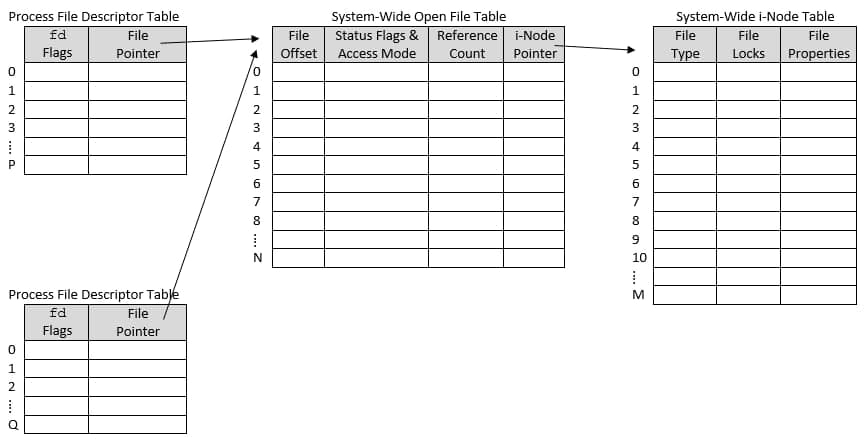
\includegraphics[width=0.85\textwidth]{fds.jpg}
    \caption{Wow such cool}
\end{figure}


\paragraph{Operazioni sugli FD: dup(), dup2()}
Libreria \texttt{unistd.h}\\
    \texttt{    int dup(int oldfd)}\\
    \texttt{    int dup2(int oldfd, int newfd)}\\ \\
Le funzioni dup() e dup2() creano una copia del file descriptor oldfd.
La funzione dup() attribuisce al nuovo file descriptor, il piu' piccolo intero non usato.
La funzione dup2() crea newfd come copia di oldfd, chiudendo prima newfd se e' necessario.

Il vecchio e nuovo file descriptor possono essere utilizzati interscambiabilmente. Essi condividono locks, puntatiori di file position e flag, ad eccezione del flag close-on-exec.
Per Esempio e' possibile effettuare una lseek() su un file descriptor e ritorvarsi la posizione modificata su entrami i file descriptor. 



\paragraph{Esempio 4: dup e dup2}\hfill \break
\lstinputlisting[language=C]{Cap1/esempio4_dup.c}

\paragraph{Esempio: (non ha file C)}
Stai scrivendo un programma shell e vuoi che ridiriga stdin e stdout in un processo figlio. Dovrebbe assomigliare a:
\begin{lstlisting}[language=C]
fdin = open(infile, O_RDONLY);
fdout = open(outfile, O_WRONLY);
// Check for errors, send messages to stdout.
...
int pid = fork();
if(pid == 0) {
    close(STDIN_FILENO);
    dup2(fdin, STDIN_FILENO);

    close(STDOUT_FILENO);
    dup2(fdout, STDOUT_FILENO);
    
    execvp(program, argv);
}
// Parent process cleans up, maybe waits for child.
...
\end{lstlisting}

\subsubsection{Permessi}
Libreria \texttt{sys/stat.h e fcntl.h}\\
%cosa sono i permessi e a cosa servono
%comandi ed esempi
Sebbene ci siano già molte buone funzionalità di sicurezza integrate nei sistemi basati su Linux, può esistere una potenziale vulnerabilità quando viene concesso l'accesso locale, ossia problemi basati sui \textbf{permessi dei file dovuti} da un utente che non assegna i permessi corretti a file e directory.
\paragraph{Proprietà dei file Linux}
Ad ogni file e directory sul tuo sistema Unix / Linux vengono assegnati \textbf{3 tipi di proprietario}:
\begin{itemize}
    \item \textbf{(u) User - Utente è il proprietario del file. } Per impostazione predefinita, la persona che ha creato un file diventa il suo\textbf{ proprietario (owner)}.
    \item \textbf{(g) Group - Gruppo di utenti può contenere più utenti. Tutti gli utenti che appartengono a un gruppo avranno le stesse autorizzazioni del gruppo Linux per accedere al file.} Supponi di avere un progetto in cui un numero di persone richiede l'accesso a un file. Invece di assegnare manualmente le autorizzazioni a ciascun utente, è possibile aggiungere tutti gli utenti a un gruppo e assegnare l'autorizzazione del gruppo al file in modo che solo i membri del gruppo e nessun altro possano leggere o modificare i file.
    \item \textbf{(o) Other - Qualsiasi altro utente che abbia accesso a un file.} Questa persona non ha creato il file, né appartiene a un gruppo utenti che potrebbe possedere il file. In pratica, significa tutti gli altri. Pertanto, quando si imposta l'autorizzazione per gli altri, viene anche definita autorizzazioni impostate per il mondo.
\end{itemize}
Come fa Linux a distinguere tra questi tre tipi di utente in modo che un \textit{utente "A" non possa influenzare un file che contiene informazioni / dati vitali di altri utenti "B"}? È come se non volessi che il tuo collega, che lavora sul tuo computer Linux, visualizzi le tue immagini. È qui che si inseriscono le autorizzazioni e definiscono il comportamento dell'utente.
\paragraph{Autorizzazioni}
Ogni file e directory nel tuo sistema UNIX / Linux ha i seguenti \textbf{3 permessi definiti per tutti e 3 i proprietari discussi sopra.}
\begin{itemize}
    \item \textbf{(r) Read - Lettura}: questa autorizzazione ti dà l'\textbf{autorità di aprire e leggere un file}. Il permesso di lettura su una directory ti dà la possibilità di elencarne il contenuto.
    \item \textbf{(w) Write - Scrittura}: l'autorizzazione di scrittura consente di \textbf{modificare il contenuto di un file}. L'autorizzazione di scrittura su una directory ti dà l'autorità per aggiungere, rimuovere e rinominare i file archiviati nella directory. Si consideri uno scenario in cui è necessario l'autorizzazione di scrittura sul file ma non l'autorizzazione di scrittura sulla directory in cui è archiviato il file. Potrai modificare il contenuto del file. Ma non sarai in grado di rinominare, spostare o rimuovere il file dalla directory.
    \item \textbf{(x) Execute - Esegui}: in Windows, un programma eseguibile di solito ha un'estensione ".exe" e che puoi eseguire facilmente. In Unix / Linux, non è possibile eseguire un programma a meno che non sia impostata l'autorizzazione di esecuzione. Se l'\textbf{autorizzazione di esecuzione} non è impostata, potresti comunque essere in grado di vedere / modificare il codice del programma (a condizione che siano impostati i permessi di lettura e scrittura), ma non eseguirlo.
\end{itemize}

\paragraph{Metodo testuale}
Scomodo, leggi la wiki se interessato.
\label{sec:permessi}
\paragraph{Metodo numerico}
L'utilizzo dei numeri è un altro metodo che consente di modificare le autorizzazioni per tutti e tre i proprietari, i gruppi e altri contemporaneamente, nonché i bit setuid, setgid e sticky. Questa struttura di base del codice è questa:

\texttt{$\$$ chmod xxx nome file}

Dove xxx è un numero di 3 cifre dove ogni cifra può essere qualsiasi cifra da 0 a 7. La prima cifra si applica alle autorizzazioni per il proprietario, la seconda cifra si applica alle autorizzazioni per il gruppo e la terza cifra si applica alle autorizzazioni per tutti gli altri.

Esempio:
\texttt{$\$$ chmod 754 filename} |
7 -$>$ Owner | 5 -$>$ Group | 4 -$>$ Others

\begin{table}[ht]
    \centering
    \begin{tabular}{c|c|c}\textbf{}
     \textbf{Number} &\textbf{ Permission Type } & \textbf{Symbol} \\
     \hline
     0 & No Permission & --- \\
    1 &	Execute & --x \\
    2 &	Write &	-w-\\
    3 &	Execute + Write & -wx\\
    4 &	Read & r--\\
    5 &	Read + Execute & r-x\\
    6 &	Read + Write & rw-\\
    7 &	Read + Write + Execute & rwx\\
    
    
\end{tabular}
    \caption{Numeri dei permessi}
    \label{tab:permessi}
\end{table}





\href{https://wiki.archlinux.org/title/File_permissions_and_attributes}{wiki} |
\href{https://www.guru99.com/file-permissions.html}{info permessi} |
\href{https://www.linux.com/training-tutorials/understanding-linux-file-permissions/}{altre info sui permessi}\\\newline
\textbf{chmod(), chown()}
\begin{itemize}
    \item \textbf{chmod()} - change mode - modifica i permessi di file e directory
    \item \textbf{chown()} - change owner - modifica il proprietario e/o il gruppo assegnato di uno o più file e directory
\end{itemize}

\begin{lstlisting}[language=C]
    int chown(const char *pathname, uid_t owner, gid_t group)
    int fchown(int fd, uid_t owner, gid_t group)
    int chmod(const char *pathname, mode_t mode)
    int fchmod(int fd, mode_t mode)
\end{lstlisting}
La differenza tra chown e fchown consiste che il primo modifica i permessi del file dal suo percorso, il secondo dal suo Process Id (fd), allo stesso modo per chmod e fchmod.

\paragraph{Esempio 5: chown e chmod}\hfill \break
\lstinputlisting[language=C]{Cap1/esempio5_chown.c}

La funziona chmod() funziona anche con i permessi numerici! 

\subsubsection{Eseguire programmi - correggere libreria e spiegare - dividere i programmi in 'esempi' e formattare meglio}
Libreria \texttt{unistd.h} -- \href{https://linuxhint.com/exec_linux_system_call_c/}{info utili}
\begin{lstlisting}[language=C]
    int execv(const char *path, char *const argv[])
    int execvp(const char *file, char *const argv[])
    int execvpe(const char *file, char *const argv[],
        char *const envp[])
    int execl(const char *path, const char *arg0,...,argn,NULL)
    int execlp(const char *file, const char *arg0,...,argn,NULL)
    int execle(const char *file, const char *arg0,...,argn, NULL,
        char *const envp[])
    int execve(const char *filename, char *const argv[], 
        char *const envp[])
\end{lstlisting}

\paragraph{Esempio 6: execv() }\hfill \break
\lstinputlisting[language=C]{Cap1/esempio6_execv1.c}
\lstinputlisting[language=C]{Cap1/esempio6_execv2.c}

\paragraph{Esempio 7: execle()} \hfill \break
\lstinputlisting[language=C]{Cap1/esempio7_execle1.c}
\lstinputlisting[language=C]{Cap1/esempio7_execle2.c}

\paragraph{Esempio 8: dup2/exec}\hfill \break
\lstinputlisting[language=C]{Cap1/esempio8_dup2_exec.c}

\paragraph{Esempio 9: chiamare la shell, system()}\hfill \break
Se si accede alle cartelle con system bisogna stare attenti perche' si vedono da root.
\lstinputlisting[language=C]{Cap1/esempio9_system.c}
\lstinputlisting[language=C]{Cap1/esempio9_system_copy.c}


\subsection{Fork}
La chiamata di sistema \textbf{Fork viene utilizzata per creare un nuovo processo, chiamato processo figlio, che viene eseguito contemporaneamente al processo che effettua la chiamata fork()} (processo genitore). Dopo aver creato un nuovo processo figlio, entrambi i processi eseguiranno l'istruzione successiva che segue la chiamata di forking. Un processo figlio utilizza lo stesso PC (Program Counter), gli stessi registri della CPU e gli stessi file utilizzati nel processo genitore.

Non accetta parametri e restituisce un valore intero. I valori restituiti dal fork() sono:
\begin{itemize}

    \item \textbf{Valore negativo}: la creazione di un processo figlio \textbf{non è riuscita}.
    \item \textbf{Zero}: \textbf{restituito al processo figlio appena creato}.
    \item \textbf{Valore positivo}: restituito \textbf{al genitore o al chiamante}. Il valore contiene l'\textbf{ID del processo figlio appena creato}.
\end{itemize}

Se la creazione del figlio ha \textbf{successo entrambi i processi ricevono un valore di ritorno}, ma questo è diverso nei due casi:
\begin{itemize}
    \item Il processo padre riceve come valore il nuovo PID del processo figlio
    \item Il processo figlio riceve come valore 0
\end{itemize} 

\href{https://www.geeksforgeeks.org/fork-system-call/}{LINK ALTRE INFO}

\subsubsection{Identificativi dei processi}
\textbf{Ad ogni processo è associato un identificativo univoco per istante temporale}, sono organizzati gerarchicamente (padre-figlio) e suddivisi in insiemi principali (sessioni) e secondari (gruppi). Anche gli utenti hanno un loro identificativo e ad ogni processo ne sono abbinati due: quello reale e quello effettivo (di esecuzione).
\begin{itemize}
    \item PID - Process ID
    \item PPID - Parent Process ID
    \item SID - Session ID
    \item PGID - Process Group ID
    \item UID/RUID - (Real) User ID
    \item EUID - Effective User ID
\end{itemize}
\paragraph{getpid(), getppid()}\hfill \break\\
\texttt{pid$\_$t getpid() : restituisce il PID del processo attivopid$\_$t}\\ 
\texttt{getppid() : restituisce il PID del processo padre}

\paragraph{Esempio 10: getpid e getppid}\hfill \break
\lstinputlisting[language=C]{Cap1/esempio10_getppid_getpid.c}

\subsubsection{Relazione tra i processi}
I processi padre-figlio:
\begin{itemize}
    \item \textbf{Conoscono reciprocamente il loro PID} (ciascuno conosce il proprio tramite getpid(), il figlio conosce quello del padre con \textbf{getppid()}, il padre conosce quello del figlio come valore di ritorno di fork())
    \item Si possono usare altre syscall per semplici interazioni come \texttt{wait e waitpid }
    \item Eventuali variabili definite prima del fork sono valorizzate allo stesso modo in entrambi: se riferiscono risorse (ad Esempio un “file descriptor” per un file su disco) fanno riferimento esattamente alla stessa risorsa.
\end{itemize} 

\subsubsection{Processi zombie e orfani}
\paragraph{wait(), waitpid()}
Librerie usate: \texttt{sys/types.h> e <sys/wait.h>}\\

La funzione \texttt{wait()} \textbf{sospende il processo corrente finche' un figlio (child) termina} o finche' il processo corrente riceve un segnale di terminazione o un segnale che sia gestito da una funzione.
Quando un \textbf{child termina il processo, senza che il parent abbia atteso la sua terminazione} attraverso la funzione di wait(), allora il child assume lo \textbf{stato di "zombie" } ossia di processo "defunto".
Se il processo corrente \textbf{esegue la funzione di wait(), in presenza di child in stato di zombie, allora la funzione ritorna immediatamente e ciascuna risorsa del child viene liberata.}

La funzione \texttt{waitpid()} \texttt{sospende il processo corrente finche' il figlio (child) corrispobndente al pid passato in argomento termina} o finche' il processo corrente riceve un segnale di terminazione o un segnale che sia gestito da una funzione.
Se il processo corrente \textbf{esegue la funzione di waitpid() e il child identificato dal pid e' in stato di zombie, allora la funzione ritorna immediatamente e ciascuna risorsa del child viene liberata} (\href{https://stackoverflow.com/questions/20688982/zombie-process-vs-orphan-process}{altre info sui processi zombie}).\\

Il valore del pid puo' essere uno dei seguenti:
\begin{itemize}
    \item -n ($<$-1: attende un qualunque figlio il cui “gruppo” è $|$-n$|$) 
    \item -1 (attende un figlio qualunque)
    \item 0 (attende un figlio con lo stesso “gruppo” del padre)
    \item n (n$>$0: attende il figlio il cui pid è esattamente n)
\end{itemize}

Se \textbf{status non e' NULL, le funzioni wait() e waitpid() memorizzano l'informazione dello stato nell'area di memoria puntata da questo argomento}.\\

Comandi utili:
\begin{lstlisting}[language=C]
    wait(st) corrisponde a waitpid(-1, st, 0)
    while(wait(NULL)>0); # attende tutti i figli    
\end{lstlisting}

Sono disponibili alcune \textbf{macro} per la valutazione dello stato status: 
\begin{itemize}
    \item \textbf{WEXITSTATUS(sts)}: restituisce lo stato vero e proprio (ad Esempio il valore usato nella “exit”)
    \item \textbf{WIFCONTINUED(sts)}: true se il figlio ha ricevuto un segnale
    \item \textbf{SIGCONTWIFEXITED(sts)}: true se il figlio è terminato normalmente
    \item \textbf{WIFSIGNALED(sts)}: true se il figlio è terminato a causa di un segnale non gestito
    \item \textbf{WIFSTOPPED(sts)}: true se il figlio è attualmente in stato di “stop”
    \item \textbf{WSTOPSIG(sts)}: numero del segnale che ha causato lo “stop” del figlio
    \item \textbf{WTERMSIG(sts)}: numero del segnale che ha causato la terminazione del figlio
\end{itemize}

\paragraph{Esempio 11: forking multiplo}\hfill \break
\lstinputlisting[language=C]{Cap1/esempio11_forking_multiplo.c}

\paragraph{Esempio 12: fork$\&$wait}\hfill \break
\lstinputlisting[language=C]{Cap1/esempio12_fork_wait.c}


\clearpage
\section{Segnali}

I \textbf{segnali} sono una forma limitata di \textbf{comunicazione inter-processo (IPC).} Un segnale è una \textbf{notifica asincrona inviata a un processo} o a un thread specifico all'interno dello stesso processo \textbf{per notificarlo di un evento}.

Ci sono vari eventi che possono avvenire in maniera asincrona al normale flusso di un programma, alcuni dei quali in maniera inaspettata e non predicibile. Per Esempio, durante l'esecuzione di un programma ci può essere una richiesta di terminazione o di sospensione da parte di un utente, la terminazione di un processo figlio o un errore generico.

Quando viene inviato un segnale, \textbf{il sistema operativo interrompe il normale flusso di esecuzione del processo di destinazione per fornire il segnale}. Se il processo ha precedentemente registrato un gestore di segnali, quella routine viene eseguita. In caso contrario, viene eseguito il gestore del segnale predefinito.\\
Per ogni processo, all'interno della process table, vengono mantenute due liste:
\begin{itemize}
    \item \textbf{Pending signals}: \textbf{segnali emessi che il processo dovrà gestire} - sono segnali nello stato "D" (\textbf{uninterruptible sleep}). Solitamente perche' il processo e' in attesa (tipo di I/O). Questo sonno non puo' essere interrotto, nemmeno sigkill (da terminale \texttt{kill -9}) puo'. Il kernel attende che il processo si "risvegli" e il segnale viene consegnato.
    \item \textbf{Blocked signals}: \textbf{segnali non comunicati al processo}. Ad ogni schedulazione del processo le due liste vengono controllate per consentire al processo di reagire nella maniera più adeguata.
\end{itemize}
\begin{table}[ht]
    \centering
    \begin{tabular}{c|c|c}\textbf{}
     \textbf{SIGXXX} &\textbf{description} & \textbf{default} \\ \\\ 
     \textbf{SIGALRM} & \textit{alarm} \textit{clock} & quit \\
     \textbf{SIGCHLD} & \textit{child} \textit{terminated} &ignore \\
     \textbf{SIGCONT} & \textit{continue, if stopped} & ignore \\
     \textbf{SIGINT} & \textit{terminal interrupt, CTRL + C} & quit \\
     \textbf{SIGKILL} & \textit{kill process}& quit \\
     \textbf{SIGSYS} & \textit{bad argument to syscall} & quit with dump \\
     \textbf{SIGTERM} & \textit{software termination} & quit \\ 
     \textbf{SIGUSR1/2 }& \textit{user signal 1/2} & quit \\
     \textbf{SIGSTOP} & \textit{stopped} & quit \\
     \textbf{SIGTSTP} & \textit{terminal stop, CTRL + Z} & quit
\end{tabular}
    \caption{Alcuni Segnali}
    \label{tab:my_label}
\end{table}

\subsection{Gestione dei segnali}
I segnali sono \textbf{simili agli interrupt}, con la differenza che gli interrupt sono mediati dal processore e gestiti dal kernel mentre \textbf{i segnali sono mediati dal kernel e gestiti dai processi}. 
Come per gli interrupts, \textbf{il programma può decidere come gestire l'arrivo di un segnale} (presente nella \textbf{lista pending}):
\begin{itemize}
    \item \textbf{Eseguendo l'azione default}
    \item \textbf{Ignorandolo} (non sempre possibile) → programma prosegue normalmente
    \item \textbf{Eseguendo un handler personalizzato} → programma si interrompe
\end{itemize}

\subsection{Default handler}
Ogni segnale ha un suo handler di default che tipicamente può:
\begin{itemize}
    \item Ignorare il segnale
    \item Terminare il processo
    \item Continuare l'esecuzione (se il processo era in stop)
    \item Stoppare il processo
\end{itemize}

\textbf{Ogni processo può sostituire il gestore di default con una funzione “custom”} (a parte per \texttt{SIGKILL e SIGSTOP}) e comportarsi di conseguenza. La sostituzione avviene tramite la \textbf{system call \texttt{signal()}}\newline\newline
Libreria \texttt{“signal.h”} $|$ \href{https://www.tutorialspoint.com/c_standard_library/c_function_signal.htm}{Info Libreria}. $\|$ \href{https://linux.die.net/man/2/signal}{LINUXDIE}
    \paragraph{signal() system call}\hfill \break
\begin{lstlisting}[language=C]
    sighandler_t signal(int signum, sighandler_t handler);
    typedef void (*sighandler_t)(int);
\end{lstlisting}

\paragraph{Esempio 13: signal()}\hfill \break
\lstinputlisting[language=C]{Cap2/esempio13_signal.c}

\paragraph{Esempio 14: (premo CTRL+C durante l'esecuzione)}\hfill \break
\lstinputlisting[language=C]{Cap2/esempio14_premiCtrlC.c}

\paragraph{Esempio 15:} \hfill \break
\lstinputlisting[language=C]{Cap2/esempio15_CST.c}
\lstinputlisting[language=C]{Cap2/esempio15_DFL.c}
\lstinputlisting[language=C]{Cap2/esempio15_IGN.c}

\subsection{Custom Handler}
Un handler personalizzato deve essere una funzione di tipo void che accetta come argomento un intero, il quale rappresenta il segnale catturato. Questo consente l'utilizzo di uno stessa handler per segnali differenti.\\
\begin{lstlisting}[language=C]
    #include <signal.h> <stdio.h> //param.c
    void myHandler(int sigNum){
        if(sigNum == SIGINT) printf("CTRL+C\n");
        else if(sigNum == SIGTSTP) printf("CTRL+Z\n");
    }
    signal(SIGINT,myHandler); 
    signal(SIGTSTP,myHandler);
\end{lstlisting}
    \paragraph{signal() return} Signal() restituisce un riferimento all'handler che era precedentemente assegnato al segnale:
\begin{itemize}
    \item NULL: handler precedente era l'handler di default
    \item 1: l'handler precedente era SIG$\_$IGN
    \item address: l'handler precedente era *(address)
\end{itemize}
\paragraph{Esempio 6:}\hfill \break
\lstinputlisting[language=C]{Cap2/esempio16.c}

\paragraph{Esempio 17: oggi, riguardare i process ID di padre e figlio se metto printf("$\%$d",child);}\hfill \break
\lstinputlisting[language=C]{Cap2/esempio17.c}

\subsection{Inviare i segnali: kill()}

\paragraph{kill()} 
\texttt{int kill(pid$\_$t pid, int sig);}\\
Invia un segnale ad uno o più processi a secondo dell'argomento pid:
\begin{itemize}
    \item pid $>$ 0: segnale al processo con PID=pid
    \item pid = 0: segnale ad ogni processo dello stesso gruppo
    \item pid = -1: segnale ad ogni processo possibile (stesso UID/RUID)
    \item pid $<$ -1: segnale ad ogni processo del gruppo |pid|Restituisce 0 se il segnale viene inviato, -1 in caso di errore.
\end{itemize}
Ogni tipo di segnale può essere inviato, non deve essere necessariamente un segnale corrispondente ad un evento effettivamente avvenuto!
\paragraph{Esempio 8:}\hfill \break
\lstinputlisting[language=C]{Cap2/esempio18.c}

\href{https://aljensencprogramming.wordpress.com/2014/05/15/the-kill-function-in-c/}{altri esempi} \\
\href{https://stackoverflow.com/questions/6501522/how-to-kill-a-child-process-by-the-parent-process}{come uccidere un figlio dal processo genitore}
\paragraph{Kill da bash} kill è un programma bash che accetta come primo argomento il tipo di segnale e come secondo argomento il PID del processo. Per maggiori info (da terminale) \texttt{man kill} per info su kill, \texttt{man signal} per informazioni sui segnali.\\
\paragraph{Esempio 19:}\hfill \break
\lstinputlisting[language=C]{Cap2/esempio19.c}

\subsection{Programmare un alarm: alarm()}
\texttt{unsigned int alarm(unsigned int seconds);}\\
La funzione alarm () viene utilizzata per generare un segnale SIGALRM dopo che è trascorso un periodo di tempo specificato.

La funzione richiede come argomento i secondi. Dopo che sono trascorsi tot secondi dalla richiesta della funzione alarm(), viene generato il segnale SIGALRM. Il comportamento predefinito al ricevimento di SIGALRM è di terminare il processo. Ma possiamo catturare e gestire il segnale come preferiamo.

La funzione alarm() restituirà un valore diverso da zero, se un altro allarme è stato precedentemente impostato e il valore è il numero di secondi rimanenti per il precedente avviso programmato dovuto alla consegna. Altrimenti alarm() restituirà zero.\\
\href{https://linuxhint.com/sigalarm_alarm_c_language/}{altri esempi e un po' di WIKI} $\|$ \href{https://www.man7.org/linux/man-pages/man2/alarm.2.html}{MANPAGE}

\paragraph{Esempio 20:}\hfill \break
\lstinputlisting[language=C]{Cap2/esempio20_alarm.c}

\paragraph{Esempio 21:}\hfill \break
\lstinputlisting[language=C]{Cap2/esempio21.c}

\subsection{Mettere in pausa: pause()}
\texttt{int pause();}
Sospende l'esecuzione del thread chiamante. Il thread non riprende l'esecuzione finché non viene consegnato un segnale e viene eseguito un gestore di segnale o terminato il thread.

Se un segnale non bloccato in arrivo termina il thread, pause() non torna mai al chiamante. Se un segnale in arrivo è gestito da un gestore di segnali, pause() ritorna dopo che il gestore di segnali è tornato.

Se pause () ritorna, restituisce sempre -1 e imposta errno su EINTR, indicando che un segnale è stato ricevuto e gestito con successo.

\href{https://www.ibm.com/docs/en/zos/2.1.0?topic=functions-pause-suspend-process-pending-signal}{da IBM} $\|$ \href{https://man7.org/linux/man-pages/man2/pause.2.html}{MANPAGE}

\paragraph{Esempio 22:}\hfill \break
\lstinputlisting[language=C]{Cap2/esempio22_pause.c}

\subsection{Bloccare i segnali}
Si considera la lista dei “blocked signals”, i segnali ricevuti dal processo ma volutamente non gestiti.

Mentre i segnali ignorati non saranno mai gestiti, i segnali bloccati sono solo temporaneamente non gestiti. Un segnale bloccato rimane nello stato \textit{pending} fino a quando esso non \textbf{viene gestito} oppure il suo handler tramutato in ignore. L'insieme dei segnali bloccati è detto \textbf{"signal mask”, una maschera dei segnali che è modificabile attraverso} la system call \texttt{sigprocmask()}\\ \href{https://www.gnu.org/software/libc/manual/html_node/Process-Signal-Mask.html}{altre info} | \href{https://www.man7.org/linux/man-pages/man2/sigprocmask.2.html}{MANPAGE}

\paragraph{sigset$\_$t} 
Una signal mask può essere gestita con un \texttt{sigset$\_$t}, una lista di segnali modificabile con alcune funzioni (non modificano maschera dei segnali del processo).
\begin{table}[ht]
    \begin{tabular}{l|l}\textbf{}
int sigemptyset(sigset$\_$t *set); & Svuota \\
int sigfillset(sigset$\_$t *set);  & Riempie \\
int sigaddset(sigset$\_$t *set, int signo); & Aggiunge singolo  \\
int sigdelset(sigset$\_$t *set, int signo); & Rimuove singolo \\
int sigismember(const sigset$\_$t *set, int signo); & Interpella
\end{tabular}
    \caption{Alcune funzioni \texttt{sigset$\_$t}}
\end{table}

\paragraph{sigprocmask()}
\texttt{int sigprocmask(int how, const sigset$\_$t *restrict set, sigset$\_$t *restrict oldset);}\\
A seconda del valore di how e di set, la maschera dei segnali del processo viene cambiata. Nello specifico:
\begin{itemize}
    \item \textbf{how = SIG$\_$BLOCK}: i segnali in set sono aggiunti alla maschera;
    \item \textbf{how = SIG$\_$UNBLOCK}: i segnali in set sono rimossi dalla maschera;
    \item \textbf{how = SIG$\_$SETMASK}: set diventa la maschera.
\end{itemize}
Se oldset non è nullo, in esso verrà salvata la vecchia maschera. oldset viene riempito anche se set è nullo.\\
\href{https://www.ibm.com/docs/en/ztpf/1.1.0.15?topic=apis-sigprocmaskexamine-change-blocked-signals}{da IBM, leggere assolutamente}\\
\paragraph{Esempio 23:}\hfill \break
\lstinputlisting[language=C]{Cap2/esempio23.c}

\paragraph{Esempio 24:}\hfill \break
\lstinputlisting[language=C]{Cap2/esempio25_sigpending.c}

\subsection{Verificare pending signals: sigpending()}
\texttt{sigpending()} restituisce l'insieme di segnali che sono in attesa di consegna al thread chiamante (cioè, i segnali che sono stati ricevuti mentre erano bloccati).\\
\paragraph{Esempio 25:}\hfill \break
\lstinputlisting[language=C]{Cap2/esempio24_sigpromask.c}

\paragraph{sigaction() - sintetizzare}
%da sintetizzare
Esamina e modifica l'azione associata a un segnale specifico.

int sig è il numero di un segnale riconosciuto. sigaction () esamina e imposta l'azione da associare a questo segnale. Vedere la Tabella 1 per i valori di sig, nonché i segnali supportati dai servizi z / OS® UNIX. L'argomento sig deve essere una delle macro definite nel file di intestazione signal.h.

const struct sigaction * new può essere un puntatore NULL. In tal caso, sigaction () determina semplicemente l'azione attualmente definita per gestire sig. Non cambia questa azione. Se new non è NULL, dovrebbe puntare a una struttura sigaction. L'azione specificata in questa struttura diventa la nuova azione associata a sig.

struct sigaction * old punta a una posizione di memoria in cui sigaction () può memorizzare una struttura sigaction. sigaction () utilizza questa posizione di memoria per memorizzare una struttura sigaction che descrive l'azione attualmente associata a sig. old può anche essere un puntatore NULL, nel qual caso sigaction () non memorizza queste informazioni.

Questa funzione è supportata solo in un programma POSIX.
Comportamento speciale per C ++:

    Il comportamento quando si combina la gestione del segnale con la gestione delle eccezioni C ++ non è definito. Inoltre, l'uso della gestione del segnale con costruttori e distruttori non è definito.
    Le convenzioni di collegamento del linguaggio C ++ e C non sono compatibili e pertanto sigaction () non può ricevere puntatori a funzione C ++. Se si tenta di passare un puntatore a funzione C ++ a sigaction (), il compilatore lo contrassegna come errore. Pertanto, per utilizzare la funzione sigaction () nel linguaggio C ++, è necessario assicurarsi che le routine di gestione dei segnali stabilite abbiano un collegamento C, dichiarandole come "C" esterno.

\href{https://www.ibm.com/docs/en/zos/2.4.0?topic=functions-sigaction-examine-change-signal-action}{da IBM}$|$\href{https://linux.die.net/man/2/sigaction}{linux.die.net}

\begin{lstlisting}[language=C]
    int sigaction(int signum, const struct sigaction *restrict act,
    struct sigaction *restrict oldact);
    
    struct sigaction {
        void (*sa_handler)(int);
        void (*sa_sigaction)(int, siginfo_t *, void *);
        sigset_t sa_mask; //Signals blocked during handlerint sa_flags; 
        //modify behaviour of signal
        void (*sa_restorer)(void); //Deprecated
\end{lstlisting}

\paragraph{Esempio 26:}\hfill \break
\lstinputlisting[language=C]{Cap2/esempio26_sigaction.c}

\paragraph{Esempio 27: blocking signal}\hfill \break
\lstinputlisting[language=C]{Cap2/esempio27.c}

\paragraph{Esempio 28: blocking signal} \hfill \break
\lstinputlisting[language=C]{Cap2/esempio28.c}

\paragraph{Esempio 29: sa$\_$sigaction}\hfill \break\lstinputlisting[language=C]{Cap2/esempio29.c}



\paragraph{easter egg} Trova le applicazioni per signal.h (\href{http://manpages.ubuntu.com/manpages/trusty/man7/signal.h.7posix.html}{UBUNTU MAN PAGE})

\clearpage
\section{Gruppi di processi}
\subsection{Gestione processi in Unix}
All'interno di Unix i processi vengono raggruppati secondi vari criteri, dando vita a sessioni, gruppi e threads.
I process groups consentono una migliore gestione dei segnali e della comunicazione tra i processi. Un processo, per l'appunto, può:
\begin{itemize}
    \item Aspettare  che  tutti  i  processi  figli  appartenenti  ad  un determinato  gruppo terminino;
    \item Mandare un segnale a tutti i processi appartenenti ad un determinato gruppo.
\end{itemize}
Esempio di utilizzo dei gruppi:
\begin{lstlisting}[language=C]
    waitpid(-33,NULL,0); // Wait for a children in group 33
    kill(-33,SIGTERM); // Send SIGTERM to all children in group 33
\end{lstlisting}
Mentre, generalmente, una sessione è collegata ad un terminale, i processi vengono raggruppati nel seguente modo:
\begin{itemize}
    \item In bash, processi concatenati tramite pipes appartengono allo stesso gruppo: \begin{verbatim}
    cat /tmp/ciao.txt | wc -l | grep '2'
    \end{verbatim}
    \item Alla loro creazione, i figli di un processo ereditano il gruppo del padre
    \item Inizialmente, tutti i processi appartengono al gruppo di 'init', ed ogni processo può cambiare il suo gruppo in qualunque momento.
\end{itemize} 
Il processo il cui PID è uguale al proprio GID è detto process group leader.

\subsection{Group System Calls}
\texttt{int setpgid(pid$\_$t pid, pid$\_$t pgid); //set GID of proc. (0=self)} \href{https://www.man7.org/linux/man-pages/man3/setpgid.3p.html}{MANPAGE}\\
La funzione setpgid() deve unirsi a un processo esistente
o creare un nuovo gruppo di processi all'interno della sessione di
processo di chiamata.

L'ID del gruppo di processi di un leader di sessione non deve cambiare.

In caso di completamento con esito positivo, l'ID del gruppo di processi che corrisponde a pid deve essere impostato su pgid.

Dopo il completamento con successo, setpgid() restituirà 0; altrimenti,
-1 e errno deve essere impostato per indicare l'errore.\\
       
\texttt{pid$\_$t getpgid(pid$\_$t pid); // get GID of process (0=self)} \href{https://www.man7.org/linux/man-pages/man3/getpgid.3p.html}{MANPAGE}\\
La funzione getpgid() restituirà l'ID del gruppo di processi del file
processo il cui ID processo è uguale a pid. Se pid è uguale a 0,
getpgid() restituirà l'ID del gruppo di processi della chiamata
processi.

Dopo il completamento con successo, getpgid() restituirà il process ID del gruppo. Altrimenti, restituirà (pid$\_$t) -1 e imposterà errno per indicare l'errore. \\
 \paragraph{Esempio 30:}\hfill \break
\lstinputlisting[language=C]{Cap3/esempio30.c}

\paragraph{Esempio 31, Mandare segnali ai gruppi:}\hfill \break
\lstinputlisting[language=C]{Cap3/esempio31.c}

\begin{enumerate}
    \item Processo 'ancestor' crea un figlioa.Il figlio cambia il proprio gruppo e genera 3 figli (Gruppo1)b.I 4 processi aspettano fino all'arrivo di un segnale
    \item Processo 'ancestor' crea un secondo figlioa.Il figlio cambia il proprio gruppo e genera 3 figli (Gruppo2)b.I 4 processi aspettano fino all'arrivo di un segnale
    \item Processo 'ancestor' manda due segnali diversi ai due gruppi
\end{enumerate}


\paragraph{Esempio 32, Wait figli in un gruppo:}\hfill \break
\lstinputlisting[language=C]{Cap3/esempio32.c}

\href{https://linux.die.net/man/2/setpgid}{more info}

\clearpage
\section{Pipe e FIFO}
    \subsection{Error in C}
    Durante l'esecuzione di un programma ci possono essere diversi tipi di errori: 
    \begin{itemize}
        \item system calls che falliscono
        \item divisioni per zero
        \item problemi di memoria
        \item ...
    \end{itemize}
    Alcuni di questi errori non fatali, come una system call che fallisce, possono essere indagati attraverso la variabile \texttt{errno}. Questa variabile globale contiene l'ultimo codice di errore generato dal sistema. 
    
    Libreria utilizzata: \texttt{errno.h} - \href{https://www.tutorialspoint.com/c_standard_library/errorno_h.htm}{DOC1}
    
    Usiamo le funzioni:
    \begin{itemize}
        \item \texttt{char *strerror(int errnum)} converte il codice di errore in una stringa comprensibile
        \item \texttt{void perror(const char *str)} stampa su stderr la stringa passatagli come argomento e vi prepende l'output di strerror
    \end{itemize}
    
    La libreria presenta anche delle variabili globali che rappresentano il tipo d'errore:
    \begin{itemize}
        \item \textbf{EDOM} - rappresenta un errore di dominio, che si verifica se un argomento di input è esterno al dominio (esempio 1)
        \item \textbf{ERANGE} - rappresenta un errore di intervallo, che si verifica se un argomento di input è al di fuori dell'intervallo (esempio 2)
        \item \href{https://www.ibm.com/docs/en/zos/2.1.0?topic=files-errnoh}{altre macro (IBM)}
    \end{itemize}
 \paragraph{Esempio 33 - EDOM} \hfill \break{}   
 \lstinputlisting[language=C]{Cap4/esempio33.c}
 
\paragraph{Esempio 34 - ERANGE} \hfill \break{}
\lstinputlisting[language=C]{Cap4/esempio34.c}
    
    \paragraph{Esempio 35: errore apertura file} \hfill \break{}
\lstinputlisting[language=C]{Cap4/esempio35.c}
    
    \paragraph{Esempio 36: errore processo non esistente}
    \lstinputlisting[language=C]{Cap4/esempio36.c}
    \subsection{Piping (def)}
    Una pipeline o data pipeline, è un insieme di elementi di elaborazione dati collegati in serie, dove l'output di un elemento è l'input di quello successivo. Gli elementi di una pipeline vengono spesso eseguiti in parallelo o in modo suddiviso nel tempo. 
    
    Si possono utilizzare le Pipe concatenando programmi tramite $\|$ in fase di chiamata.

\paragraph{Esempio 37: utilizzo di una pipe} \hfill
    \lstinputlisting[language=C]{Cap4/esempio37A.c}
    \lstinputlisting[language=C]{Cap4/esempio37b.c}
 
    \subsection{Pipe anonime}
        %def
        Una pipe anonima è un canale di \textbf{comunicazione FIFO}  che può essere utilizzato per la comunicazione interprocesso (IPC) \textbf{unidirezionale}. Un'implementazione è spesso integrata nel sottosistema di I / O file del sistema operativo. 
        
        In genere un programma padre apre pipe anonime e crea un nuovo processo che eredita le altre estremità delle pipe o crea diversi nuovi processi e li dispone in una pipeline. Il collegamento avviene utilizzando \textbf{file  descriptors} (motivo per cui serve l'antenato comune).
        
        Libreria utilizzata: \texttt{unistd.h}
        \subsubsection{Creazione e scrittura di pipe - pipe()}
        Funzione: \texttt{int pipe (int pipefd[2])}
        
        La funzione pipe crea una pipe e inserisce i descrittori di file per le estremità di lettura e scrittura della pipe (rispettivamente) in pipefd[0] e pipefd[1] (corrispondono a stdin e stdout).

         In caso di esito positivo, la pipe restituisce 0; in caso di errore, restituisce -1. I codici di errore \texttt{errno} sono:
    \begin{itemize}
        \item \textbf{EMFILE} Il processo ha troppi file aperti.
        \item \textbf{ENFILE} Sono presenti troppi file aperti nell'intero sistema.
    \end{itemize}

    \paragraph{Esempio 38: Creazione pipe} \hfill \break{}
\lstinputlisting[language=C]{Cap4/esempio38.c}
    
    \subsubsection{Lettura di pipe - read()}
    \texttt{int read(int fd[0],char * data, int num)}\\
    Tenta di leggere fino al conteggio dei byte dal descrittore di file fd nel buffer a partire da buf.
    Sui file che supportano la ricerca, l'operazione di lettura inizia dall'offset del file.
        
    
    La lettura della pipe tramite il comando read restituisce valori differenti a seconda della situazione:
    \begin{itemize}
        \item In caso di successo restituisce il numero di bytes effettivamente letti
        \item Se il lato di scrittura è stato chiuso (da ogni processo) ed il buffer è vuoto restituisce 0
        \item Se il buffer è vuoto ma il lato di scrittura è ancora aperto (in qualche processo) il processo si sospende fino alla disponibilità dei dati o alla chiusura
        \item Se si provano a leggere più bytes (num) di quelli disponibili, vengono recuperati solo quelli presenti
        \item In caso di errore, viene restituito -1 e viene impostato \texttt{errno}.
    \end{itemize}
    \href{https://man7.org/linux/man-pages/man2/read.2.html}{MANPAGE}
    
    \paragraph{Esempio 39: lettura pipe}\hfill \break
    \lstinputlisting[language=C]{Cap4/esempio39.c}
    
    \subsubsection{Lettura pipe - write()}
       
    \texttt{int write(int fd[0],char * data, int num)}
    
    La funzione \texttt{write()} scrive i dati da un buffer dichiarato dall'utente su un determinato dispositivo, come un file. E' il modo principale per produrre dati da un programma utilizzando direttamente una chiamata di sistema. La destinazione è identificata da un codice numerico. I dati da scrivere, ad esempio un pezzo di testo, sono definiti da un puntatore e da una dimensione, espressa in numero di byte. \href{https://en.wikipedia.org/wiki/Write_(system_call)}{WIKI}
    
    \begin{table}[ht]
    \centering
    \begin{tabular}{c|l}\textbf{}
    \textbf{Argument} &	\textbf{Description} \\ \\
    \textbf{fd} & It is the file descriptor which has been obtained from the call to open. It is an integer \\ 
     & value. The values 0, 1, 2 can also be given, for standard input, standard output $\&$ \\ 
     & standard error, respectively . \\
    \textbf{data} & It points to a character array, with content to be written to the file pointed to by fd. \\
    \textbf{num} & It specifies the number of bytes to be written from the character array into the \\
     & file pointed to by fd.\\ 
\end{tabular}
    \caption{Argomenti \texttt{write()}}
    \label{tab:tab3}
\end{table}
\subsection{Gestione dei segnali}
    
    
    \texttt{int fcntl(int fd, cmd, arg;}
    Letteralmente \textbf{File Control}.
    
    Apre il descrittore di file fd. Può accettare un terzo argomento opzionale. \href{https://man7.org/linux/man-pages/man2/fcntl.2.html}{MANPAGE}
    \newline

\begin{table}[ht]
    \centering
    \begin{tabular}{c l}
    \textbf{F$\_$DUPFD} 
            &    duplica il descrittore di file fd usando il numero più basso descrittore di file \\
            &    disponibile maggiore o uguale a arg. Questo è diverso da dup2 (2), che utilizza \\
            &    esattamente l'estensione descrittore di file specificato. In caso di successo, \\
            &    viene restituito il nuovo descrittore di file. \\
    
    \textbf{F$\_$GETFD} & Restituisce (come risultato della funzione) i flag del descrittore \\
            &    di file; arg viene ignorato. \\
    
    \textbf{F$\_$SETFD} & Imposta i flag del descrittore di file sul valore specificato da\\
            &   arg. \\
    
\end{tabular}
    \caption{Alcuni cmd}
    \label{tab:tab4}
\end{table}
    
    \paragraph{Esempio 40: comunicazione bidirezionale} \hfill \break
    Un tipico esempio di comunicazione unidirezionale tra un processo scrittore P1 ed un processo lettore P2 è il seguente:
    \begin{enumerate}
        \item P1 crea una pipe()
        \item P1 esegue un fork() e crea P2
        \item P1 chiude il lato lettura: close(fd[0])
        \item P2 chiude il lato scrittura: close(fd[1])
        \item P1 e P2 chiudono l'altro fd appena finiscono.
    \end{enumerate}
    \lstinputlisting[language=C]{Cap4/esempio40.c}
    
    \paragraph{Esempio 41: bidirezionale}\hfill \break
    Un tipico esempio di comunicazione bidirezionale tra un processo scrittore P1 ed un processo lettore P2 è il seguente:
    \begin{enumerate}
        \item P1 crea duepipe(), pipe1 e pipe2
        \item P1 esegue un fork() e crea P2
        \item P1 chiude il lato lettura di pipe1 ed il lato scrittura di pipe2
        \item P2 chiude il lato scrittura di pipe1 ed il lato lettura di pipe2
        \item P1 e P2 chiudono gli altri fd appena finiscono di comunicare.
    \end{enumerate}
    \lstinputlisting[language=C]{Cap4/esempio41.c}
    
    \subsubsection{Gestire la comunicazione}
    Per gestire comunicazioni complesse c'è bisogno di definire un “protocollo”, ad esempio:
    \begin{itemize}
        \item Messaggi di lunghezza fissa (magari inviata prima del messaggio)
        \item Marcatore di fine messaggio (per esempio con carattere NULL o newline)Più in generale occorre definire la sequenza di messaggi attesi
    \end{itemize}

    \paragraph{Esempio 42:-MAYBE ERR- redirige lo stdout di cmd1 sullo stdin di cmd2} \hfill \break
 \lstinputlisting[language=C]{Cap4/esempio42.c}

    \subsection{Pipe con nome (FIFO)}
        %def
    Le pipe con nome, o FIFO, corrispondono a dei file speciali nel filesystem grazie ai quali i processi, senza vincoli di gerarchia, possono comunicare. Un processo può accedere ad una di queste pipe se ha i permessi sul file corrispondente ed è vincolato, ovviamente, all'esistenza del file stesso.Essendo oggetti nel file system, si possono usare le funzioni di scrittura/lettura dei file viste nelle scorse lezioni. Una volta creata una pipe con nome, il file associato è persistente!NB: al contrario di un normale file, una FIFO deve essere aperta da entrambi i lati per potervi interagire in modo ragionevole.
        \subsubsection{Esempio 43: Creazione Pipe}
        \texttt{int mkfifo(const char *pathname, mode$\_$t mode);} %SPIEGARE LA FUNZIONE MKFIFO
            \lstinputlisting[language=C]{Cap4/esempio43.c}
            \paragraph{Esempio 44: writer} \hfill \break
               \lstinputlisting[language=C]{Cap4/esempio44.c}
            
            \paragraph{Esempio 45: reader}\hfill \break
               \lstinputlisting[language=C]{Cap4/esempio44.c}
            
\clearpage
\section{Message Queue and Threads}
    %atm sto copiando le slide del prof, poi aggiungo spiegazioni extra - like always
    Una  coda  di  messaggi,  message  queue,  è  una  lista  concatenata  memorizzata all'interno  del  kernel  ed  identificata  con  una  chiave  (un  intero  positivo  univoco), chiamata queue identifier. Questa  chiave  viene  condivisa  tra  i  processi  interessati,  i  quali  generano  degli ulteriori identificativi da usare durante l'interazione con la coda.Una  coda  deve  essere  innanzitutto  generata  in  maniera  analoga  ad  una  FIFO, impostando dei permessi. Ad una coda esistente si possono aggiungere o recuperare messaggi tipicamente in modalità “autosincrona”: la lettura attende la presenza di un messaggio, la scrittura attende che via sia spazio disponibile. Questi comportamenti possono però essere configurati.
    
    \subsection{Queues}
        \subsubsection{Struttura del messaggio}
        Ogni messaggio inserito nella coda ha tre campi:
        \begin{itemize}
            \item Un tipo (intero “long”)
            \item Una lunghezza non negativa
            \item Un insieme di dati (bytes) di lunghezza corretta
        \end{itemize}
        
        Al contrario delle FIFO, i messaggi in una coda possono essere recuperati anche sulla base del tipo e non solo del loro ordine “assoluto” di arrivo. Così come i files, le code sono delle strutture persistenti che continuano ad esistere, assieme ai messaggi in esse salvati, anche alla terminazione del processo che le ha create. L'eliminazione deve essere esplicita.
        
        \begin{lstlisting}[language=C]
struct msg_buffer{
    long mtype;
    char mtext[100];
} message;
        \end{lstlisting}
        \href{https://www.ibm.com/docs/en/aix/7.1?topic=files-msgh-file}{IBM} - \href{https://www.man7.org/linux/man-pages/man0/sys_msg.h.0p.html}{MANPAGE}
        \subsubsection{Creazione coda}
        Funzione \texttt{int msgget(key$\_$t key, int msgflg)}\\
        
        \href{https://man7.org/linux/man-pages/man2/msgget.2.html}{MANPAGE} Restituisce l'identificativo di una coda basandosi sulla chiave “key” e sui flags:
        \begin{itemize}
            \item \textbf{IPC$\_$CREAT}: crea una coda se non esiste già, altrimenti restituisce l'identificativo di quella già esistente
            \item \textbf{IPC$\_$EXCL}: (da usare assieme al precedente) fallisce se coda già esistente
            \item \textbf{0xxx}: numero ottale di \hyperref[sec:permessi]{permessi}, analogo a quello che si può usare nel file system 
        \end{itemize}
        
        In caso di successo, il valore restituito sarà l'identificatore della coda dei messaggi (un numero intero non negativo), altrimenti -1 con errno che indica l'errore.

        \begin{lstlisting}[language=C]
#include <sys/types.h> <sys/ipc.h> <sys/msg.h> /msgget.c
key_t queueKey = 56; //Unique key
int queueId = msgget(queueKey, 0777 | IPC_CREAT | IPC_EXCL);
        \end{lstlisting}
        
        \subsubsection{Ottenere una chiave univoca}
        Funzione \texttt{key$\_$t ftok(const char *pathname, int proj$\_$id) }. \\
        
        \href{https://man7.org/linux/man-pages/man3/ftok.3.html}{MANPAGE} Restituisce  una  chiave  basandosi  sul path  (una  cartella  o  un  file),  esistente  ed accessibile nel file-system, e sull'id numerico. La chiave dovrebbe essere univoca e sempre la stessa per ogni coppia $<path,id>$ in ogni istante sullo stesso sistema.Un metodo d'uso, per evitare possibili conflitti, potrebbe essere generare un path (es. un file) temporaneo univoco, usarlo, eventualmente rimuoverlo, ed usare l'id per per rappresentare diverse “categorie” di code, a mo' di indice.
        
        \texttt{key$\_$t ftok(const char *path, int id)}
        
        \begin{lstlisting}[language=C]
#include <sys/ipc.h> //ftok.c
key_t queue1Key = ftok("/tmp/unique", 1);
key_t queue2Key = ftok("/tmp/unique", 2); ...
        \end{lstlisting}
        
            \paragraph{Esempio 46: creazione}\hfill \break
\lstinputlisting[language=C]{Cap5/esempio46.c}
        \subsubsection{Persistenza delle code}
        Se eseguiamo questo programma dopo aver eseguito il precedente \textit{ipcCreation.c} verrà generato un errore dato che la coda esiste già ed abbiamo usato il flag \textbf{IPC$\_$EXCL}!
            \paragraph{Esempio 47: le queue sono persistenti}\hfill \break
        \lstinputlisting[language=C]{Cap5/esempio47.c}
        \subsubsection{Inviare messaggi}
        \texttt{int msgsnd(int msqid, const void *msgp, size$\_$t msgsz, int msgflg);}\\
        
        \href{https://linux.die.net/man/2/msgsnd}{LINUX.DIE} Aggiunge  un  messaggio  di  dimensione msgsz alla  coda  identificata  da msquid, puntata  dal  buffer msgp.  Il  messaggio  viene  inserito  immediatamente  se  c'è abbastanza spazio disponibile, altrimenti la chiamata si blocca fino a che abbastanza spazio diventa disponibile. Se msgflg è \textbf{IPC$\_$NOWAIT} allora la chiamata fallisce in assenza di spazio.
        
        \subsubsection{Ricevere messaggi}
        \texttt{ssize$\_$t msgrcv(int msqid,void *msgp,size$\_$t msgsz,long msgtyp,int msgflg)}\\

        \href{https://linux.die.net/man/2/msgsnd}{LINUX.DIE} Rimuove un messaggio dalla coda msqid e lo salva nel buffer msgp. msgsz specifica la lunghezza  massima  del  testo  del  messaggio  (mtext  della  struttura msgp).  Se  il messaggio  ha  una  lunghezza  maggiore  e  \textit{msgflg}  è  \textbf{MSG$\_$NOERROR}  allora  il messaggio viene troncato (viene persa la parte in eccesso), se \textbf{MSG$\_$NOERROR} non è specificato allora il messaggio non viene eliminato e la chiamata fallisce. A seconda di \textit{msgtyp} viene recuperato il messaggio:
        \begin{itemize}
            \item \textit{msgtyp} = 0: primo messaggio della coda
            \item \textit{msgtyp} $>$ 0: primo messaggio di tipo \textit{msgtyp}, o primo messaggio di tipo diverso da \textit{msgtyp} se \textbf{MSG\_EXCEPT} è impostato come flag
            \item \textit{msgtyp} $<$ 0: primo messaggio il cui tipo T è \texttt{min(T<=|msgtyp|)}. In fine, il flag \textbf{IPC\_NOWAIT} fa fallire la syscall se non sono presenti messaggi (altrimenti hang)
        \end{itemize}

            \paragraph{Esempio 48: comunicazione}\hfill \break
        \lstinputlisting[language=C]{Cap5/esempio48.c}
        \subsubsection{Modificare la coda}
        \texttt{int msgctl(int msqid, int cmd, struct msqid$\_$ds *buf);}\\
        
        \href{https://man7.org/linux/man-pages/man2/msgctl.2.html}{MANPAGE} Modifica la coda identificata da \textit{msqid} secondo i comandi cmd, riempiendo buf con informazioni  sulla  coda  (ad  esempio  tempo  di  ultima  scrittura,  di  ultima  lettura, numero messaggi nella coda, etc...). I valori per cmd sono:
        \begin{itemize}
            \item \textbf{IPC$\_$STAT}: recupera informazioni da kernel
            \item \textbf{IPC$\_$SET}: imposta alcuni parametri a seconda di buf
            \item \textbf{IPC$\_$RMID}: rimuove immediatamente la coda
            \item \textbf{IPC$\_$INFO}: recupera informazioni generali sui limiti delle code nel sistema
            \item \textbf{MSG$\_$INFO}: come \textbf{IPC$\_$INFO} ma con informazioni differenti
            \item \textbf{MSG$\_$STAT}: come \textbf{IPC$\_$STAT} ma con informazioni differenti
        
        \end{itemize}

            \paragraph{msqid$\_$ds structure}\hfill \break
        \begin{lstlisting}[language=C]
struct msqid_ds {
  struct ipc_perm msg_perm; /* Ownership and permissions */
  time_t msg_stime; /* Time of last msgsnd(2) */
  time_t msg_rtime; /* Time of last msgrcv(2) */
  time_t msg_ctime; //Time of creation or last modification by msgctl
  unsigned long msg_cbytes; /* # of bytes in queue */
  msgqnum_t msg_qnum; /* # of messages in queue */
  msglen_t msg_qbytes; /* Maximum # of bytes in queue */
  pid_t msg_lspid; /* PID of last msgsnd(2) */
  pid_t msg_lrpid; /* PID of last msgrcv(2) */
};
        \end{lstlisting}
            \paragraph{ipc$\_$perm structure}\hfill \break
        \begin{lstlisting}[language=C]
 struct ipc_perm {
   key_t __key; /* Key supplied to msgget(2) */
   uid_t uid; /* Effective UID of owner */
   gid_t gid; /* Effective GID of owner */
   uid_t cuid; /* Effective UID of creator */
   gid_t cgid; /* Effective GID of creator */
   unsigned shortmode; /* Permissions */
   unsigned short __seq; /* Sequence number */
 };     
        \end{lstlisting}
        \paragraph{Esempio 49: modifica}\hfill \break
        \lstinputlisting[language=C]{Cap5/esempio49.c}
    \subsection{Threads}
    I thread sono singole sequenze di esecuzione all'interno di un processo, aventi alcune delle proprietà dei processi. Non sono indipendenti tra loro: condividono il codice, i dati e le risorse del sistema assegnate al processo di appartenenza. Come ogni singolo processo hanno alcuni elementi indipendenti, come lo stack, il PC ed i registri del sistema. La creazione di threads consente un parallelismo delle operazioni in maniera rapida e semplificata. Context switch tra threads è rapido, così come la loro creazione, terminazione e comunicazione.
    
    Per la compilazione è necessario aggiungere il flag \texttt{-pthread} \\  ad esempio:texttt{gcc -o program main.c -pthread}
        \subsubsection{Creazione}
        In C i thread corrispondono a delle funzioni eseguite in parallelo al codice principale. Ogni thread è identificato da un ID e può essere gestito come un processo figlio, con funzioni che attendono la sua terminazione.
            \begin{lstlisting}[language=C]
int pthread_create(
    pthread_t *restrict thread, /* Thread ID */
    const pthread_attr_t *restrict attr, /* Attributes */
    void *(*start_routine)(void *), /* Function to be executed */
    void *restrict arg /* Parameters to above function */
);
            \end{lstlisting}
            \paragraph{Esempio 50: Creazione}\hfill \break
            \lstinputlisting[language=C]{Cap5/esempio50.c}
        \subsubsection{Terminazione}
Un nuovo thread termina in uno dei seguenti modi:

        \begin{itemize}
            \item Chiamando la funzione noreturn void pthread$\_$exit(void *retval); specificando un puntatore di ritorno.
            \item Ritorna dalla funziona associata al thread specificando un valore di ritorno.
            \item Viene cancellato
            \item Qualche thread chiama exit(), o il thread che esegue main() ritorna dallo stesso, terminando così tutti i threads.
        \end{itemize}

        \subsubsection{Cancellazione Thread}
        \texttt{int pthread$\_$cancel(pthread$\_$t thread);} \\
        
        Invia una richiesta di cancellazione al thread specificato, il quale reagirà (come e quando)  a  seconda  di  due  suoi  attributi: state e type. State può  essere enabled(default) o disabled: se disabled la richiesta rimarrà in attesa fino a che state diventa enabled, se enabled la cancellazione avverrà a seconda di type. Type può essere deferred (default) o asynchronous: attende la chiamata di un cancellation point o termina  in  qualsiasi  momento,  rispettivamente.  Cancellation  points  sono  funzioni definite nella libreria pthread.h (lista). State e typepossono essere modificati:\\ \\
        \texttt{int pthread$\_$setcancelstate(int state, int *oldstate);}
        
        Con state = PTHREAD$\_$CANCEL$\_$DISABLE o PTHREAD$\_$CANCEL$\_$ENABLE 
        \\ \\
        \texttt{int pthread$\_$setcanceltype(int type, int *oldtype);}
        
        Con type = PTHREAD$\_$CANCEL$\_$DEFERRED o PTHREAD$\_$CANCEL$\_$ASYNCHRONOUS
            \paragraph{Esempio 51: Creazione e cancellazione}\hfill \break
            \lstinputlisting[language=C]{Cap5/esempio51.c}
        \subsubsection{Aspettare un Thread}
        Un processo (thread) che avvia un nuovo thread può aspettare la sua terminazione mediante la funzione:\\ 
        \texttt{int pthread$\_$join(pthread$\_$t thread, void **retval);}\\
        Che ritorna quando il thread identificato da thread termina, o subito se il thread è già terminato. Se il valore di ritorno del thread non è nullo (parametro di pthread$\_$exit o di return), esso viene salvato nella variabile puntata da retval. Se il thread era stato cancellato, retval è riempito con PTHREAD$\_$CANCELED.Solo se il thread è joinable può essere aspettato! Un thread può essere aspettato da al massimo un thread!
            \paragraph{Esempio 52: Join 1}\hfill \break
            \lstinputlisting[language=C]{Cap5/esempio52.c}
            \paragraph{Esempio 53: Join 2}\hfill \break
            \lstinputlisting[language=C]{Cap5/esempio53.c}
            \paragraph{Esempio 54: Join 3}\hfill \break
            \lstinputlisting[language=C]{Cap5/esempio54.c}
        Ogni thread viene creato con degli attributi specificati nella struttura pthread$\_$attr$\_$t. Questa struttura, analogamente alla struttura usata per gestire le maschere dei segnali, è un oggetto usato solo alla creazione di un thread, ed è poi indipendente dallo stesso (se cambia,  gli  attributi  del  thread  non  cambiano).  La  struttura  va  inizializzata  con int  pthread$\_$attr$\_$init(pthread$\_$attr$\_$t  *attr); che  imposta  tutti  gli attributi al loro valore di default. Una volta usata e non più necessaria, la struttura va distrutta con     int pthread$\_$attr$\_$destroy(pthread$\_$attr$\_$t *attr);I vari attributi della struct possono, e devono, essere modificati singolarmente con le seguenti funzioni:int pthread$\_$attr$\_$setxxxx(pthread$\_$attr$\_$t *attr, params);int pthread$\_$attr$\_$getxxxx(const pthread$\_$attr$\_$t *attr, params);
        
        \begin{itemize}
            \item ...detachstate(pthread$\_$attr$\_$t *attr, int detachstate)
                \begin{itemize}
                    \item PTHREAD$\_$CREATE$\_$DETACHED -> non può essere aspettato
                    \item PTHREAD$\_$CREATE$\_$JOINABLE -> default, può essere aspettato
                    \item Può essere cambiato durante l'esecuzione con int pthread$\_$detach(pthread$\_$t thread);
                \end{itemize}
            \item ...sigmask$\_$np(pthread$\_$attr$\_$t *attr,const sigset$\_$t *sigmask);
            \item ...affinity$\_$np(...)
            \item ...setguardsize(...)
            \item ...inheritsched(...)
            \item ...schedparam(...)
            \item ...schedpolicy(...)
            \item altri
        \end{itemize}

        \subsubsection{Detached e joinable threads}
         I threads vengono creati di default nello stato joinable, il che consente ad un altro thread di attendere la loro terminazione attraverso il comando pthread$\_$join. I thread joinable rilasciano le proprie risorse non alla terminazione ma quando un thread fa il join con loro (salvando lo stato di uscita) (così come i sottoprocessi), oppure alla terminazione del processo. Contrariamente, i thread in stato detached liberano le loro risorse immediatamente una volta terminati, ma non consentono ad altri processi di fare il “join”.NB:  un  thread  detached  non  può  diventare  joinable  durante  la  sua  esecuzione, mentre il contrario è possibile.
            \paragraph{Esempio 55: Attributi}\hfill \break
            \lstinputlisting[language=C]{Cap5/esempio55.c}
%\section*{Unnumbered Section}



\clearpage
\section{Esercizi}
\subsection{Cap1}
Scrivere dei programmi in C che:
\begin{itemize}
    \item Avendo come argomenti dei “binari”, si eseguono con exec ciascuno in un sottoprocesso (*)
    \item idem punto 1 ma in più salvando i flussi di stdout e stderr in un unico file (*)
    \item Dati due eseguibili come argomenti del tipo ls e wc si eseguono in due processi distinti: il primo deve generare uno stdout redirezionato su un file temporaneo, mentre il secondo deve essere lanciato solo quando il primo ha finito leggendo lo stesso file come stdin.Ad esempio ./main ls wc deve avere lo stesso effetto di ls $|$ wc.
\end{itemize}

Suggerimenti: anziché due figli usare padre-figlio- usare dup2 per far puntare il file descriptor del file temporaneo su stdout in un processo e stdin nell'altro sfruttare wait per attendere la conclusione del processo che genera l’output\\(*) generando DUE figli.

\clearpage
\section{Link utili}
\begin{itemize}
  \item \tt{\href{https://digilander.libero.it/uzappi/C/librerie/C-unistd.html}{libreria unistd.h}}
  \item \href{http://manpages.ubuntu.com/manpages/trusty/man7/signal.h.7posix.html}{signal.h da DOC Ubuntu}
  \item \href{https://www.geeksforgeeks.org/signals-c-language/}{esempi di signal in C -- da implementare nel doc}
  \item \href{https://www.tutorialspoint.com/c_standard_library/c_function_signal.htm}{signal.h in C}
  \item \href{https://www.computerhope.com/unix/signals.htm}{codici segnali }
\end{itemize}
\end{document}
